\vspace*{0pt}
\begin{multicols}{2}
\topic{Feed Forward Neural Network}
\textbf{Question:} Assume that the neurons have a sigmoid activation function. Perform a forward pass on the given network and also calculate error.

\begin{tikzpicture}[
    node distance=1.5cm,
    neuron/.style={circle, draw, minimum size=8mm, font=\small},
    weight/.style={font=\scriptsize},
]

% Nodes
\node[neuron] (x1) at (0,0) {$x_1$};
\node[neuron, below=of x1] (x2) {$x_2$};

\node[neuron, right=2cm of x1] (h1) {$h_1$};
\node[neuron, below=of h1] (h2) {$h_2$};
\node[weight, above=4mm] at (h1) {$b_1 = 0.25$};

\node[neuron, right=2cm of h1] (o1) {$o_1$};
\node[neuron, below=of o1] (o2) {$o_2$};
\node[weight, above=4mm] at (o1) {$b_2 = 0.35$};

\draw[<-, >=stealth] (x1) -- ++(-0.8,0) node[left] {$0.1$};
\draw[<-, >=stealth] (x2) -- ++(-0.8,0) node[left] {$0.5$};

\draw[->, >=stealth] (o1) -- ++(0.8,0) node[right] {$0.5$};
\draw[->, >=stealth] (o2) -- ++(0.8,0) node[right] {$0.95$};


% Connections with weights
\draw[->, >=stealth] (x1) -- (h1) node[weight, midway, above] {$w_{1}=0.1$};
\draw[->, >=stealth] (x1) -- (h2) node[weight, midway, above right, sloped] {$w_{2}=0.2$};
\draw[->, >=stealth] (x2) -- (h1) node[weight, midway, above right, sloped] {$w_{3}=0.3$};
\draw[->, >=stealth] (x2) -- (h2) node[weight, midway, above] {$w_{4}=0.4$};

\draw[->, >=stealth] (h1) -- (o1) node[weight, midway, above] {$w_{5}=0.5$};
\draw[->, >=stealth] (h1) -- (o2) node[weight, midway, above right, sloped] {$w_{6}=0.6$};
\draw[->, >=stealth] (h2) -- (o1) node[weight, midway, above right, sloped] {$w_{7}=0.7$};
\draw[->, >=stealth] (h2) -- (o2) node[weight, midway, above] {$w_{8}=0.8$};

\end{tikzpicture}

For Hidden Layer:\\[0.5em]
$\begin{aligned}
   h_{1(in)} &= w_1x_1 + w_3x_2 + b_1\\
   &= 0.1 \times 0.1 + 0.3 \times 0.5 + 0.25 = 0.41\\
   h_{1(out)} &= \sigma(h_{1(in)}) = \frac{1}{1 + e^{-0.41}} = 0.601
   \\[1em]
   h_{2(in)} &= w_2x_1 + w_4x_2 + b_1\\
   &= 0.2 \times 0.1 + 0.4 \times 0.5 + 0.25 = 0.47\\
   h_{2(out)} &= \sigma(h_{2(in)}) = \frac{1}{1 + e^{-0.47}} = 0.615\\
\end{aligned}$

\vspace{1em}
For Output Layer:\\[0.5em]
$\begin{aligned}
   o_{1(in)} &= w_5(h_{1(out)}) + w_7(h_{2(out)}) + b_2\\
   &= 0.5 \times 0.601 + 0.7 \times 0.615 + 0.35 = 1.081\\
   o_{1(out)} &= \sigma(o_{1(in)}) = \frac{1}{1 + e^{-1.081}} = 0.746
   \\[1em]
   o_{2(in)} &= w_6(h_{1(out)}) + w_8(h_{2(out)}) + b_2\\
   &= 0.6 \times 0.601 + 0.8 \times 0.615 + 0.35 = 1.2026\\
   o_{2(out)} &= \sigma(o_{2(in)}) = \frac{1}{1 + e^{-1.2026}} = 0.769\\
\end{aligned}$

\vspace{1em}
Error Calculation:\\[0.5em]
$\begin{aligned}
   \text{MSE} &= \frac{1}{2} \left[ (t_1 - o_1)^2 + (t_2 - o_2)^2 \right]\\
   &= \frac{1}{2} \left[ (0.5-0.746)^2 + (0.95-0.769)^2 \right]\\
   &= 0.0466\\
\end{aligned}$

\textbf{Question:} 
Applying back propagation, update the weights $w_{1,1}$ and $w_{1,3}$ of the back propagation neural network shown in the following figure after one epoch. Sigmoid function is-used as an activation function. Learning rate $\alpha=0.6$, actual output from node $o_3$ is $0.5$, and bias for the hidden $b_1=0.55$:


\begin{tikzpicture}[
    node distance=1.5cm,
    neuron/.style={circle, draw, minimum size=8mm, font=\small},
    weight/.style={font=\scriptsize},
]
% Nodes
\node[neuron] (x1) at (0,0) {$x_1$};
\node[neuron, below=of x1] (x2) {$x_2$};

\node[neuron, right=2.5cm of x1] (h1) {$h_1$};
\node[neuron, below=of h1] (h2) {$h_2$};
\node[weight, above=4mm] at (h1) {$b_1 = 0.55$};

\draw[<-, >=stealth] (x1) -- ++(-0.8,0) node[left] {$0.35$};
\draw[<-, >=stealth] (x2) -- ++(-0.8,0) node[left] {$0.7$};

\node[neuron, right=of h1, yshift=-1cm] (o3) {$o_3$};
\draw[->, >=stealth] (o3) -- ++(0.8,0) node[right] {$0.5$};


% Connections with weights
\draw[->, >=stealth] (x1) -- (h1) node[weight, midway, above] {$w_{1,1}=0.2$};
\draw[->, >=stealth] (x1) -- (h2) node[weight, midway, above right, sloped] {$w_{1,2}=0.3$};
\draw[->, >=stealth] (x2) -- (h1) node[weight, midway, above right, sloped] {$w_{2,1}=0.2$};
\draw[->, >=stealth] (x2) -- (h2) node[weight, midway, above] {$w_{2,2}=0.3$};

\draw[->, >=stealth] (h1) -- (o3) node[weight, midway, above,sloped] {$w_{1,3}=0.3$};
\draw[->, >=stealth] (h2) -- (o3) node[weight, midway, above,sloped] {$w_{2,3}=0.9$};
\end{tikzpicture}

For Hidden Layer:\\[0.5em]
$\begin{aligned}
   h_{1(in)} &= w_{11}x_1 + w_{21}x_2 + b_1\\
   &= 0.2 \times 0.35 + 0.2 \times 0.7 + 0.55 = 0.76\\
   h_{1(out)} &= \sigma(h_{1(in)}) = \frac{1}{1 + e^{-0.76}} = 0.68
   \\[1em]
   h_{2(in)} &= w_{12}x_1 + w_{22}x_2 + b_1\\
   &= 0.3 \times 0.35 + 0.3 \times 0.7 + 0.55 = 0.865\\
   h_{2(out)} &= \sigma(h_{2(in)}) = \frac{1}{1 + e^{-0.865}} = 0.703\\
\end{aligned}$


\vspace{1em}
For Output Layer:\\[0.5em]
$\begin{aligned}
   o_{3(in)} &= w_{13}(h_{1(out)}) + w_{23}(h_{2(out)}) + b_{2}\\
   &= 0.3 \times 0.68 + 0.9 \times 0.703 + 0 = 0.8367\\
   o_{3(out)} &= \sigma(o_{3(in)}) = \frac{1}{1 + e^{-0.8367}} = 0.697
\end{aligned}$

\vspace{1em}
Error Calculation:\\[0.5em]
MSE $= \frac{1}{2} \left[(0.5 - 0.697)^2\right]
= 0.0194$

\topic{Information Gain}
Construct the decision tree step by step, showing all calculations for Information Gain (using Entropy). Determine whether the email, where the length is long, does not contain links, and does not include attachments, is classified as spam.

\begin{tabularx}{0.47\textwidth}{|c|C|C|c|}
   \hline
   \textbf{Email Length} & \textbf{Contains Links} & \textbf{Contains Attachments} & \textbf{Spam?} \\\hline
   Short & Yes & No & Yes \\
   Long & No & Yes & No \\
   Short & Yes & Yes & Yes \\
   Long & Yes & No & No \\
   Short & No & No & No \\\hline
\end{tabularx}

Entropy of entire dataset,\\[0.5em]
$E(D) = E(2,3) = -\frac{2}{5}\log_2{\frac{2}{5}}-\frac{3}{5}\log_2{\frac{3}{5}} = 0.9709$

\pagebreak
Information Gain of Email Length,\\[0.5em]
$\begin{aligned}
&E(Short) = E(2,1) = -\frac{2}{3}\log_2{\frac{2}{3}}-\frac{1}{3}\log_2{\frac{1}{3}}  = 0.918\\
&E(Long) = E(0,2) = -0\log_2{0}-\frac{2}{2}\log_2{\frac{2}{2}} = 0\\
&IG(D, \text{Email}) = 0.9709 - \left(\frac{3}{5} \times 0.918 + \frac{2}{5} \times 0\right) = 0.4201
\end{aligned}$


Information Gain of Contains Links,\\[0.5em]
$\begin{aligned}
&E(Yes) = E(2,1) = -\frac{2}{3}\log_2{\frac{2}{3}}-\frac{1}{3}\log_2{\frac{1}{3}}  = 0.918\\
&E(No) = E(0,2) = -0\log_2{0}-\frac{2}{2}\log_2{\frac{2}{2}} = 0\\
&IG(D, \text{Links}) = 0.9709 - \left(\frac{3}{5} \times 0.918 + \frac{2}{5} \times 0\right) = 0.4201
\end{aligned}$


Information Gain of Contains Attachments,\\[0.5em]
$\begin{aligned}
&E(Yes) = E(1,1) = -\frac{1}{2}\log_2{\frac{1}{2}}-\frac{1}{2}\log_2{\frac{1}{2}}  = 1\\
&E(No) = E(1,2) = -\frac{1}{3}\log_2{\frac{1}{3}}-\frac{2}{3}\log_2{\frac{2}{3}} = 0.918\\
&IG(D, \text{Attach.}) = 0.9709 - \left(\frac{2}{5} \times 1 + \frac{3}{5} \times 0.918\right) = 0.0201
\end{aligned}$


Since, $IG(D, \text{Email Length}) = IG(D, \text{Contains Links})$ > $IG(D, \text{Contains Attachments})$, we can choose either Email Length or Contains Links as the root node.


\begin{center}
   \begin{tikzpicture}
   [node distance=1cm, >=stealth, attr/.style={circle, draw, minimum size=12mm, font=\footnotesize, align=center}]
   \node[attr] (email) {Email\\Length};
   \node[attr, below right=of email] (longno) {Not\\Spam};
   \node[attr, below left=of email] (link) {Has\\Links};
   \draw[->] (email) -- node[midway,above,sloped]{short} (link);
   \draw[->] (email) -- node[midway,above,sloped]{long} (longno);

   \node[attr, below right=of link] (linkno) {Not\\Spam};
   \draw[->] (link) -- node[midway,above,sloped]{no} (linkno);
   
   
   \node[attr, below left=of link] (yes) {Yes\\Spam};
   \draw[->] (link) -- node[midway,above,sloped]{yes} (yes);
   
   % \node[attr, below left=of link] (attach) {attach\\ment};
   % \draw[->] (link) -- node[midway,above,sloped]{yes} (attach);
   % \node[attr, below right=of link] (no) {Not\\Spam};
   % \draw[->] (link) -- node[midway,above,sloped]{yes} (no);
\end{tikzpicture}
\end{center}

If the email length is long, then it is classified as \textit{Not Spam}.

\columnbreak
\topic{CNN}
Construct the output of each layer in the CNN illustrated in Figure 2, assuming white cells represent 0 and black cells represent 1:

\begin{center}
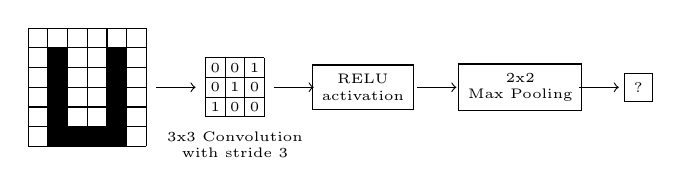
\begin{tikzpicture}
   [scale=0.25]
   \draw (0,0) grid (6,6);
   \fill[black] (1,0) rectangle (2,5);
   \fill[black] (4,0) rectangle (5,5);
   \fill[black] (2,0) rectangle (4,1);

   \draw[yshift=0.5cm] (9,1) grid ++(3,3);
   \node[font=\tiny] at (9.5,2) {1};
   \node[font=\tiny] at (9.5,3) {0};
   \node[font=\tiny] at (9.5,4) {0};
   \node[font=\tiny] at (10.5,2) {0};
   \node[font=\tiny] at (10.5,3) {1};
   \node[font=\tiny] at (10.5,4) {0};
   \node[font=\tiny] at (11.5,2) {0};
   \node[font=\tiny] at (11.5,3) {0};
   \node[font=\tiny] at (11.5,4) {1};
   \node[below, align=center, font=\tiny] at (10.5,1.25) {3x3 Convolution\\with stride 3};
   \draw[->] (6.5,3) -- ++(2,0);
   
   \node[draw, align=center, font=\tiny] at (17,3) {RELU\\activation};
   \draw[->] (12.5,3) -- ++(2,0);
   
   \node[draw, align=center, font=\tiny] at (25,3) {2x2\\Max Pooling};
   \draw[->] (19.75,3) -- ++(2,0);
   
   \node[draw, align=center, font=\tiny] at (31,3) {?};
   \draw[->] (28,3) -- ++(2,0);
\end{tikzpicture}
\end{center}

\textbf{Solution:}\\[0.5em]
Converting image to matrix form:

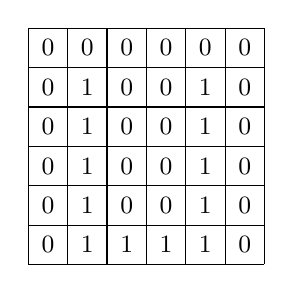
\begin{tikzpicture}
   [scale=0.5]
   \draw (0,0) grid (6,6);
   \node[font=\small] at (0.5,5.5) {0};
   \node[font=\small] at (1.5,5.5) {0};
   \node[font=\small] at (2.5,5.5) {0};
   \node[font=\small] at (3.5,5.5) {0};
   \node[font=\small] at (4.5,5.5) {0};
   \node[font=\small] at (5.5,5.5) {0};

   \node[font=\small] at (0.5,4.5) {0};
   \node[font=\small] at (1.5,4.5) {1};
   \node[font=\small] at (2.5,4.5) {0};
   \node[font=\small] at (3.5,4.5) {0};
   \node[font=\small] at (4.5,4.5) {1};
   \node[font=\small] at (5.5,4.5) {0};

   \node[font=\small] at (0.5,3.5) {0};
   \node[font=\small] at (1.5,3.5) {1};
   \node[font=\small] at (2.5,3.5) {0};
   \node[font=\small] at (3.5,3.5) {0};
   \node[font=\small] at (4.5,3.5) {1};
   \node[font=\small] at (5.5,3.5) {0};

   \node[font=\small] at (0.5,2.5) {0};
   \node[font=\small] at (1.5,2.5) {1};
   \node[font=\small] at (2.5,2.5) {0};
   \node[font=\small] at (3.5,2.5) {0};
   \node[font=\small] at (4.5,2.5) {1};
   \node[font=\small] at (5.5,2.5) {0};

   \node[font=\small] at (0.5,1.5) {0};
   \node[font=\small] at (1.5,1.5) {1};
   \node[font=\small] at (2.5,1.5) {0};
   \node[font=\small] at (3.5,1.5) {0};
   \node[font=\small] at (4.5,1.5) {1};
   \node[font=\small] at (5.5,1.5) {0};

   \node[font=\small] at (0.5,0.5) {0};
   \node[font=\small] at (1.5,0.5) {1};
   \node[font=\small] at (2.5,0.5) {1};
   \node[font=\small] at (3.5,0.5) {1};
   \node[font=\small] at (4.5,0.5) {1};
   \node[font=\small] at (5.5,0.5) {0};
\end{tikzpicture}


After 3x3 Convolution with stride 3:\\[0.5em]
$\begin{aligned}
   C_{1,1} =
   &(0 \cdot 0) + (0 \cdot 0) + (0 \cdot 1) + 
   (0 \cdot 0) + (1 \cdot 1) + (0 \cdot 0) \\ +
   &(0 \cdot 1) + (1 \cdot 0) + (0 \cdot 0) = 1 \\[0.5em]
   C_{1,2} =
   &(0 \cdot 0) + (0 \cdot 0) + (0 \cdot 1) + 
   (0 \cdot 0) + (1 \cdot 1) + (0 \cdot 0) \\ +
   &(0 \cdot 1) + (1 \cdot 0) + (0 \cdot 0) = 1 \\[0.5em]
   C_{2,1} =
   &(0 \cdot 0) + (1 \cdot 0) + (0 \cdot 1) + 
   (0 \cdot 0) + (1 \cdot 1) + (0 \cdot 0) \\ +
   &(0 \cdot 1) + (1 \cdot 0) + (1 \cdot 0) = 1 \\[0.5em]
   C_{2,2} =
   &(0 \cdot 0) + (1 \cdot 0) + (0 \cdot 1) + 
   (0 \cdot 0) + (1 \cdot 1) + (0 \cdot 0) \\ +
   &(1 \cdot 1) + (1 \cdot 0) + (0 \cdot 0) = 2 \\[0.5em]
\end{aligned}$

% $\therefore$ Output after convolution:
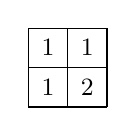
\begin{tikzpicture}
   [scale=0.5]
   \draw (0,0) grid (2,2);
   \node[font=\small] at (0.5,1.5) {1};
   \node[font=\small] at (0.5,0.5) {1};
   \node[font=\small] at (1.5,1.5) {1};
   \node[font=\small] at (1.5,0.5) {2};
\end{tikzpicture}

After Relu activation:

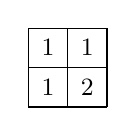
\begin{tikzpicture}
   [scale=0.5]
   \draw (0,0) grid (2,2);
   \node[font=\small] at (0.5,1.5) {1};
   \node[font=\small] at (0.5,0.5) {1};
   \node[font=\small] at (1.5,1.5) {1};
   \node[font=\small] at (1.5,0.5) {2};
\end{tikzpicture}

After 2x2 max pooling:

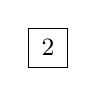
\begin{tikzpicture}
   [scale=0.5]
   \draw (0,0) grid (1,1);
   \node[font=\small] at (0.5,0.5) {2};
\end{tikzpicture}
\end{multicols}